\documentclass[11pt]{article}
\renewcommand{\baselinestretch}{1.20} 
\usepackage[utf8]{inputenc}
\usepackage[english]{babel}
\usepackage{graphicx}
\usepackage{wrapfig}
\usepackage{subcaption}
\usepackage{enumitem}
\usepackage{geometry}
\usepackage{xcolor}
\usepackage{float}
\usepackage{mdframed}
\usepackage{fancyhdr}
\usepackage{lastpage}
\usepackage{booktabs}% http://ctan.org/pkg/booktabs
\newcommand{\tabitem}{~~\llap{\textbullet}~~}
\geometry{a4paper, total={170mm,237mm}, left=20mm, top=20mm}
\setlength{\abovecaptionskip}{15pt plus 3pt minus 2pt}

\pagestyle{fancy}
\fancyhf{}
\rfoot{Side \thepage \hspace{1pt} / \pageref{LastPage}}
\begin{document}
    
    % Title page
    \begin{titlepage}
    \centering
	
\includegraphics[width=0.35\textwidth]{Projectdoc/Assets/Illustrationer/aau_logo_en.pdf}\par\vspace{1cm}
	{\scshape\Large Struktureret System Udvikling\par}
	\vspace{0.2cm}
	{\huge\bfseries Workshop 3\par}
	\vspace{0.2cm}
	{\scshape\Large ITC - B125\par}
	\vspace{2cm}
	{\Large\itshape 
    	Mikkel Steen Hansen\\
        Benjamin Bach Jensen\\
        Daniel Vestergaard Jensen\\
    \par}
	\vfill
	\vfill
\end{titlepage}
    
    % Table of contents
    \renewcommand{\baselinestretch}{0.8}
    \tableofcontents
    \renewcommand{\baselinestretch}{1.20}
    \newpage
    
    \section{Beskrivelse}
    \textbf{Mini projekt: Vejr station}\\
    %Dagens workshop omhandler at videre udvikle på sidste workshops vejr station, for anvendelse i et parcel hus. I dette workshop ligger fokus i testing og error handling.\\
    %Tanken bag projektet er at forskellige sensorer registrerer en eller flere informationer der skal til for at beskrive vejret. Disse data samles op via en enhed der kan videregive information til en app på brugerens smartphone eller computer, evt. krydret med en præcis vejrudsigt i den kommende time ved at udnytte services fra DMI eller anden vejr tjeneste.
    \noindent
    Dagens workshop omhandler testing og error handling.
    Tanken bag projektet er at gruppen har fået to funktionen SqueareRoot og BubbleSort, der nu videre skal anvendes i sammenhæng til at sotere en gruppe tal, finde et gennemsnit, de tre mindste tal, de tre største tal, og tilsidst det mest, samt det mindst tal afvigende fra gennemsnittet.\\
    %
    %\begin{figure}[H]
    %    \centering
    %    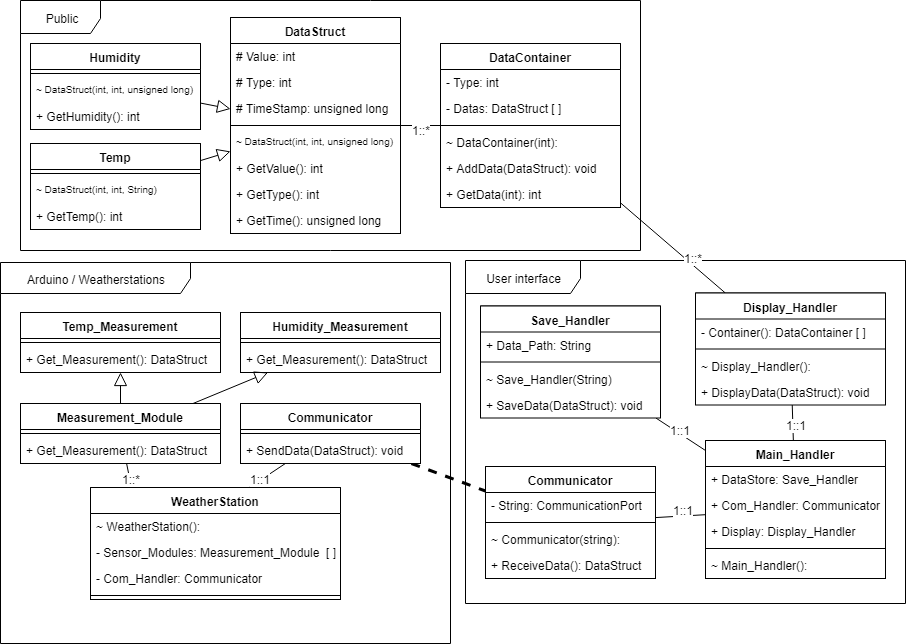
\includegraphics[width=1\textwidth,angle=0]{Struktureret_System_Udvikling/Workshop_2/Assets/Workshop2_ClassDiagram.png}
    %    \caption{Interaction Class Diagram}
    %    \label{fig:ClassDiagram}
    %\end{figure}
    %\noindent
    %Gruppen har i dette workshop valgt at lægge mest vægt på testing og handling i koden omhandlende Userinterface. Hvor her referere til sidste workshops class diagram \ref{fig:ClassDiagram}.
    %Dog forefindes stadig mindre whiteboxtesting path tests på Vejrstationens side. F.eks. kan man under Temp\_Measurement og Humidity\_Measurement finde følgende, der tester ikke kun tester den litererede path men også en minor result test.
    %
    %\begin{figure}[H]
    %    \begin{subfigure}{.35\textwidth}
    %        \centering
    %        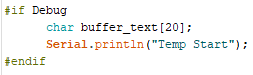
\includegraphics[width=1\linewidth]{Struktureret_System_Udvikling/Workshop_3/Assets/Start.PNG}
    %        \caption{Path testing}
    %        \label{fig:TestPath}
    %    \end{subfigure}
    %    \begin{subfigure}{.65\textwidth}
    %        \centering
    %        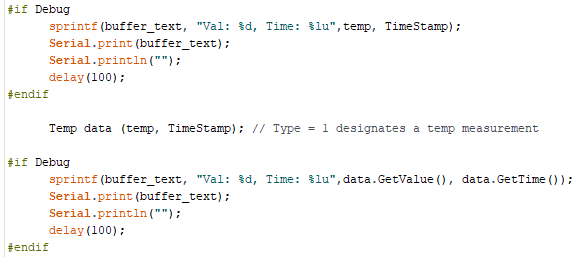
\includegraphics[width=1\linewidth]{Struktureret_System_Udvikling/Workshop_3/Assets/Secound.PNG}
    %        \caption{Minor result testing}
    %        \label{fig:TestRes}
    %    \end{subfigure}
    %    \label{fig:Testing}
    %\end{figure}
    %
    %Den anden side... pc
    %
    \noindent
    %Foruden førnævnte har gruppen også implementeret følgende funktionaliteter:
    %SquareRoot og BubbleSort.
    Dog har disse to førnævnte funktionaliteter påvist manglende test, samt returnerer ikke det forventede resultat.
    Denne konklution kan uddrages fra at udfører af en black test. En test der ikke anvender kode, men hvor gyldighed af en funktionalitens output bliver valideret,i forhold til det forventede resultat, efter en forudbestemmelse af alle mulige inputs.
    
    \newpage
    \noindent
    For SquareRoot har gruppen dannet følgende skema for mulige indputs, samt hvad disse retunerede under første gennemgang (inden rettelse), og hvad der faktisk forventes som resultat.
    \begin{center}
        \begin{tabular}{ |c|c|c| }
            \hline
             Testet input & Forventet resultat & Faktisk resultat \\
            \hline
             Bogstaver & - & - \\
              A & Ugyldigt & Endless loop with 0 as input\\
              V & Ugyldigt & Endless loop with 0 as input \\
              Å & Ugyldigt & Endless loop with 0 as input \\
              * & Ugyldigt & Endless loop with 0 as input \\
             Hele tal \textless 0 & - & - \\ 
              -2869 & Ugyldigt & Endless loop with 686467 as output,\\ 
              && before segmentation fault\\
              -4 & Ugyldigt & Endless loop with 1.33438 as output,\\ 
              && before segmentation fault \\
             Dicimal tal \textless 0 & - & -\\
              -954.459 & Ugyldigt & Endless loop with 75902.4 as output,\\ 
              && before segmentation fault\\
              -8.5 & Ugyldigt & Endless loop with 5.337551 as output,\\ 
              && before segmentation fault \\
             Tallet 0 & 0 & 0 \\
             Hele tal \textgreater 0 & - & - \\
              5625 & 75 & Endless loop with 2.63878e+006 as output,\\ 
              && before segmentation fault \\
              2869 & 53.5630469 & Endless loop with 686467 as output,\\ 
              && before segmentation fault \\
              15 & 3.8729833 & Endless loop with 18.7647 as output,\\ 
              && before segmentation fault \\
              4 & 2 & Endless loop with 1.33438 as output,\\ 
              && before segmentation fault \\
             Dicimal tal \textgreater 0 & - & - \\
              5625.5625 & 75.0037499 & Endless loop with 2.63878e+006 as output,\\ 
              && before segmentation fault \\
              2869.9682 & 53.5720841 & Endless loop with 686467 as output,\\ 
              && before segmentation fault \\
              15.51 & 3.9382737 & Endless loop with 18.7647 as output,\\ 
              && before segmentation fault \\
              4.0 & 2.0 & Endless loop with 1.33438 as output,\\ 
              && before segmentation fault \\
             \hline
        \end{tabular}
    \end{center}
    
    \newpage \noindent
    For BubbleSort har gruppen dannet følgende skema for mulige indputs, samt hvad disse retunerede under første gennemgang (inden rettelse), og hvad der forventes som resultat.
    \begin{center}
        \begin{tabular}{ |c|c|c| } 
            \hline
             Testet input & Forventet resultat & Faktisk resultat \\
            \hline
             Bogstaver & - & - \\
              CBDAFEHIG & ABCDEFGHI or & \\ 
              &65 66 67 68 69 70 71 72 73 & 67 \\
              VXURWTSZY & RSTUVWZXY or & \\ 
              & 82 83 84 85 86 87 88 89 90 & 88 \\
              ÄÅØÆëæøïå & åëïÄÅæÆøØ or & \\ 
              & 134 137 139 142 143 145 146 155 157 & -59 \\
              +\$-!/*\#\&= & !\#\$\&*+-/= or & \\
              & 33 35 36 38 42 43 45 47 61 & 43 \\
             Hele tal \textless 0 & - & - \\
              -1500 -2679 -1890 -1233 -1967 & -1233 -1456 -1500 -1785-1967 & \\
              -2255 -1456 -1785 -2122 & -1890 -2122 -2255 -2679 & -1500\\ 
              &&\\
              -4 -2 -5 -1 -3 -9 -6 -7 -8 & -1 -2 -3 -4 -5 -6 -7 -8 -9 & -2\\ 
             Dicimal tal \textless 0 & - & -\\
              -954.459 -199.991 -956.569 -2856.2750 & -199.991 -325.895 -457.835 -954.459 & \\
              -2111.1112 -2574.3567 -325.895 -457.835 & -956.569 -1046.4785 -2111.1112 -2574.3567 & \\ 
              -1046.4785 & -2856.2750 & -199 \\ 
              &&\\
              -8.5 -4.6 -2.8 -1.1 -3.2 -9.2 -6.7 -5.3 -7.4 & -1.1 -2.8 -3.2 -4.6 -5.3 -6.7 -7.4 -8.5 -9.2 & -4\\ 
             Hele tal \textgreater 0 & - & - \\
              1500 2679 1890 1233 3657 & 1111 1233 1500 1890 2679 & \\ 
              4782 3589 9999 1111 & 3589 3657 4782 9999 & 2679\\
              &&\\
              4 2 5 1 9 7 6 8 3 & 1 2 3 4 5 6 7 8 9 & 4 \\
             Dicimal tal \textgreater 0 & - & - \\
              954.459 199.991 956.569 2856.2750 & 199.991 357.428 564.249 894.352 & \\ 
              9999.1111 1111.9999 564.249 357.428 & 954.459 956.569 1111.9999 2856.2750 & \\ 
              894.352 & 9999.1111 & 954\\ 
              &&\\
              8.5 4.6 2.8 1.1 9.3 3.2 7.9 5.6 6.3 & 1.1 2.8 3.2 4.6 5.6 6.3 7.9 8.5 9.3 & 8\\ 
             Mixed Tal & - & -\\
              1 -4 5.8 -7.2 9 -9 1.5 -1 6 & -9 -7.2 -4 -1 1 1.5 5.8 6 9 & 1 \\
              2 -1  569 -204 999 -111 5 -4 0 & -204 -111 -4 -1 0 2 5 569 999 & 2\\
             \hline
        \end{tabular}
    \end{center}
    
    \newpage \noindent
    Efter disse overstående resultater har gryppen foretaget rettelser af disse to funktionaliteter ved anvendelse af whitebox testing. Dette er en testings metode, hvor funktionaliteten gennemgåes først i en flowgraf ved dens forventede outputs, for forudbestemte muligheder eller inputs, og dernæst også ved nærmere inspektion af selve koden, samt dens faktiske givende resultater.
    
    \noindent
    For SquareRoot har gruppen dannet følgende Flowgraf:\\
    \begin{table}[H]
        \begin{minipage}{.7\textwidth}
            \begin{figure}[H]
                \centering
                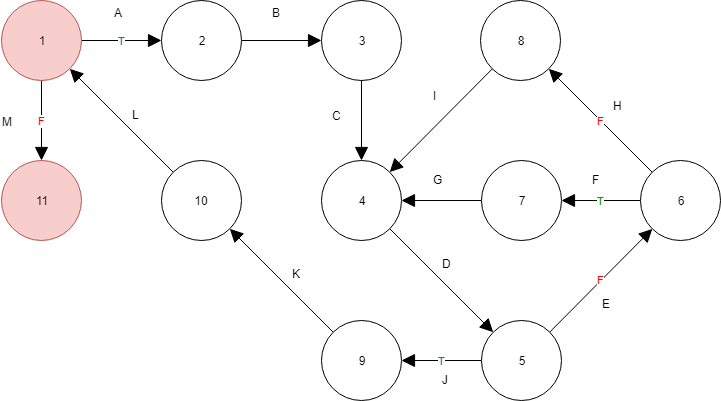
\includegraphics[width=1\textwidth,angle=0]{Struktureret_System_Udvikling/Workshop_3/SquareRoot_FlowGraph.png}
                \caption{SquearRoot FlowGraph Diagram}
                \label{fig:SquearRootGraph}
            \end{figure}
        \end{minipage}
        \begin{minipage}{.3\textwidth}
            \quad
            \begin{tabular}{lllll}
                1 & Main While loop\\
                2 & Get number input\\
                3 & SquareRoot\\
                4 & Sqrt\\
                5 & Is result found?\\
                6 & Is the guess too high?\\
                7 & Guess is too high\\
                8 & Guess is too low\\
                9 & Result found \\
                10 & Print result\\
                11 & End the program\\
            \end{tabular}
        \end{minipage}
    \end{table}
    \noindent
    Og kan derfor, ved et retmæssigt forløb forvente en gennemgang i vejene:\\
    A-B-C-\{D-E-[F-G/H-I]\}*"Nødvendige gæt"-D-J-K-L-M\\
    Hvor \{ - \} definere et loop af en vis størrelse, der altid skal opfylde det beskrevne mønster.\\
    Den eneste undvigelse kan ses ved F-G der også kan være beskrevet ved vejen H-I.\\
    \\
    Efter første gennemgang kan det konkluderes at funktionen tager følgende vej:\\
    A-B-C-D-E-F-G-D-E-F-G-D-E-F-G-.... Dette tyder på at funktionen går i loop ved funktionen "sqrt" under check på gættets størrelse i forhold til det originale tal, og herefter udprinter "To High".
    Ved nærmere inspektion kan det også fra gennemgangens output, ses at det reelt indtastede tal, som er 4 i denne test, nu er blevet til 16. En kombination af disse betyder, at tallet kun vil blive mindre, da gættet er klassificeret som værende "To High", og derved aldrig rammer det originale tal, der desuden også er blevet kvadreret.
    \begin{figure}[H]
        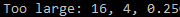
\includegraphics[width=0.3\textwidth,angle=0]{Struktureret_System_Udvikling/Workshop_3/Udklip.PNG}
        \label{fig:Udklip}
    \end{figure}
    \noindent
    Disse fejl kan rettes i funktionen SquareRoot1, hvor "res = sqrt(val*val,val/2.0,0.5);" skal rettes til "res = sqrt(val,val/2.0,0.5);" og i funktionen sqrt, hvor "if (tal+EPS \textgreater tmp)" skal rettes til "if (tal+EPS \textless tmp)".
    Efter næste gennemgang kan det dog stadig ses, at funktionen ikke tager den forventede vej, da vejen stadig er det samme loop, for det efterspurgte tal "i dette tilfælde 16". Dog kan der denne gang også ses ud fra gennemgangens udput at tredje tal "Step", hvilket bliver anvendt til at beregne næste gæt, bliver mindre og mindre.
    \begin{figure}[H]
        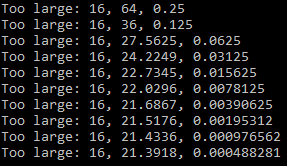
\includegraphics[width=0.3\textwidth,angle=0]{Struktureret_System_Udvikling/Workshop_3/Udklip2.PNG}
        \label{fig:Udklip2}
    \end{figure}
    \noindent
    også ved at give funktionen et andet inputs, og derved foretage vejen ...D-E-H-I istedet for ...-D-E-F-G. vil funktionen udputte det forventede resultat.
    Efter en videre inspektion af forskellen på disse kan derved konkluderes at fejlenn ligger i funktionen sqrt, i checket for om gættet er for høj, hvor "step = 0.5*step;" skal rettes til "step = 0.5;"
    
    \\
    \noindent
    For BubbleSort har gruppen dannet følgende Flowgraf:\\
    \begin{table}[H]
        \begin{minipage}{.7\textwidth}
            \begin{figure}[H]
            \centering
            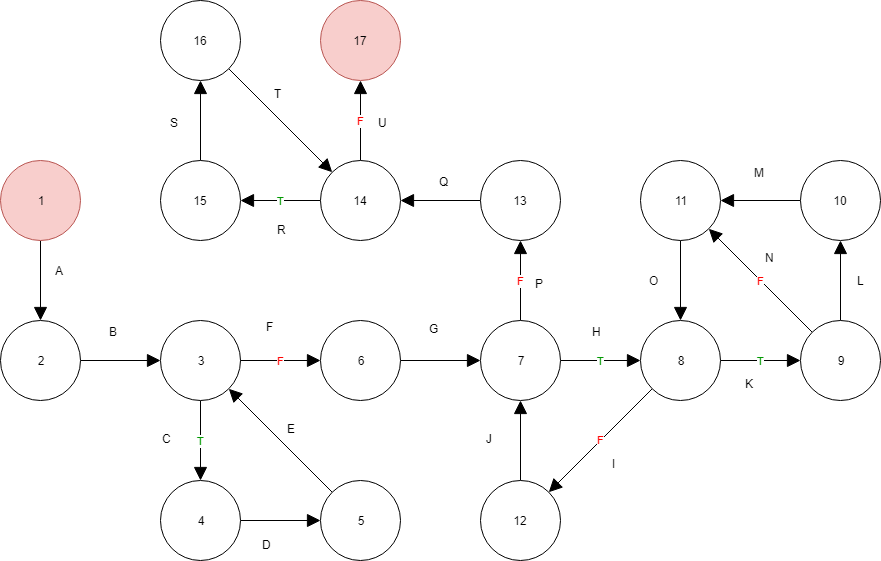
\includegraphics[width=1\textwidth,angle=0]{Struktureret_System_Udvikling/Workshop_3/Booble_Sort_Flowgraph.png}
            \caption{BoobleSort FlowGraph Diagram}
            \label{fig:BoobleSortGraph}
            \end{figure}
        \end{minipage}
        \begin{minipage}{.3\textwidth}
            \quad
            \begin{tabular}{lllll}
                1 & Before sorting\\
                2 & Print Array\\
                3 & If looped through Array\\
                4 & Print number in Array\\
                5 & Add counter in loop "Print"\\
                6 & Before Sorting\\
                7 & If looped through Array or non Switched\\
                8 & Loop through remaining unsorted Array\\
                9 & If current sorting pos is bigger then next\\
                10 & Switch number possitions\\
                11 & Add counter in loop "remaining unsorted"\\
                12 & Add counter in loop "Array or non Switched"\\
                13 & After Sorting\\
                14 & Print Array\\
                15 & If looped through Array\\
                16 & Print number in Array\\
                17 & Add counter in loop "Print"\\
            \end{tabular}
        \end{minipage}
    \end{table}
    \noindent
    Og kan derfor, ved et retmessigt forløb forvente en gennemgang i vejene:\\
    A-B-\{C-D-E\}*"Array størelse"-F-G-\{H-\{K-[N/L-M]-O\}-I-J\}-P-O-\{R-S-T\}*"Array størelse"-U\\
    Hvor \{ - \} definere et loop af en vis størelse, der altid skal opfylde det beskrævende mønster.\\
    Eneste undvigelse kan ses ved N der også kan være beskrevet ved vejen L-M.\\
    \\
    Efter første gennemgang kan dog konkluderes at funktionen tager følgende vej:\\
    A-B-\{C-D-E\}*4-F-G-H-K-K-K-K-......\\
    Derved kan ses at her forekommer 2 typer af fejl:\\
    Første i loopet mellem C,D,E der ikke fuldender den forvendtede længte. Denne kan løses ved kodens forloop der skal rettes fra "for(int i = 0; i \textless --size; i++)" til "for(int i = 0; i \textless= size; i++)".\\
    Anden fejl forekommer i loopet ved K, hvor man ved en nærmere kode inspektion kan se at de omkringliggende loops mangler afsluttende brakkets.\\
    Efter anden gennemgang kan dog stadig ses, at funktionen ikke tager forventede vej, da næste forventede vej ville være: F-G-H-K-L-M-O-K-L-M-O..., for det diffenerede array "10-2-5...", og ikke den resulterende vej: F-G-H-K-N-O-K-N-O...\\
    Denne fejl skal findes i sorterings kodens tjek for, om et ellement på den givende possition er stører end næsteværende ellement. Koden "if(a[j] \textless a[i+1])" skal derfor rettes til "if(a[j] \textgreater a[j+1])", da j diffinerer nuværende tjek og i diffinerer arrayets gennemgang. Efterfølgende skal dog også bemærkes at det samme deffinerede "i", også anvendt i koden "hold = a[i];", heller ikke relatere til den forvendtede possition, og skal derfor af samme grunde rettes til "hold = a[j];".\\
    Efter sidste gennemgangs rettelser, kan sidste fejlrettelse findes i loopet diffineret fra H-J, der ved et gennemløb bliver affsluttet inden dens forvendtede ressultat. Altså kan fejlen findes i koden "for(i = 0; i \textless (size \&\& switched); i++)", hvor her bemærkes at loopets header indeholder en forkert sat ramme "i \textless (size \&\& switched)" skal derfor rettes til "(i \textless size) \&\& switched".

    %% ved ikke helt med nederestående .......

    %\noindent
    %Nu da disse funktionaliterer er blevet rettet, og giver forventede output, kan disse efterfølgende blive anvendt i følgende støre %fonktionaliteter:
    %Gennemsnit og standardafvigelsesberegningsfunktionalitet,
    %samt Sorterings alguritme.
    %Til disse har gruppen også efterfølgende anvendt Blackbox testing, en metode hvor forventede output sammenligenes med faktuelle resultat, uden %brug af kode inspektion, for både førnævnte induviduelle funktionaliteter såvel som hele systeme, til efterfølgende kontrol tests.
    
\end{document}